\subsubsection{Increased instrument-shaft resistance}
\label{sec:shaft_resistance_results}

The parameter distributions and Pearson correlation matrices are
provided in Appendix~\ref{app:dof2}.
Across all command amplitudes, the one-cycle M1 absolute current-residual
peak ranged from 10.23 to 62.16~mA in healthy
recordings and from 96.53 to 151.04~mA in degraded recordings.

\paragraph{Cross-validation}
Table~\ref{tab:dof2-overall} presents a subset of the 113 evaluated
LDA feature sets, including the best-performing current-only models
and selected video-only and combined models.
The four runs provided 216 one-cycle observations, with 108 per class.
All command amplitudes, frequencies and waveforms were pooled, and
each complete run was held out once.

\begin{table}[t]
\centering
\caption{Selected pooled shaft LDA results using leave-one-run-out
cross-validation and one-cycle observations. Each class contains 108
observations from two runs. Green indicates no missed detections or
false alarms.}
\label{tab:dof2-overall}
{\fontsize{8.5}{10}\selectfont
\setlength{\tabcolsep}{2.5pt}
\renewcommand{\arraystretch}{1.1}
\begin{tabularx}{\columnwidth}{@{}>{\raggedright\arraybackslash}X rrrr@{}}
\toprule
\textbf{LDA input features} & TP & FN & TN & FP \\
\midrule
\multicolumn{5}{@{}l}{\textit{Current only}} \\
M1 absolute peak & \gbcorrect{108} & \gbcorrect{0} & \gbcorrect{108} & \gbcorrect{0} \\
M1 RMS & \gbcorrect{108} & \gbcorrect{0} & \gbcorrect{108} & \gbcorrect{0} \\
M1 phase mean & 73 & 35 & 108 & 0 \\
M2 phase mean & 82 & 26 & 108 & 0 \\
M2 amplitude at $2f_{\mathrm{cmd}}$ & 81 & 27 & 108 & 0 \\
\midrule
\multicolumn{5}{@{}l}{\textit{Video only}} \\
Negative gain $g_-$ & 107 & 1 & 90 & 18 \\
Absolute gain difference & 76 & 32 & 100 & 8 \\
Centred video residual MAE & 86 & 22 & 93 & 15 \\
Positive gain + negative gain & 106 & 2 & 89 & 19 \\
\midrule
\multicolumn{5}{@{}l}{\textit{Current + video}} \\
M1 absolute peak + gain difference & \gbcorrect{108} & \gbcorrect{0} & \gbcorrect{108} & \gbcorrect{0} \\
M1 phase mean + gain difference & 102 & 6 & 107 & 1 \\
M2 amplitude at $2f_{\mathrm{cmd}}$ + gain difference & 81 & 27 & 106 & 2 \\
\bottomrule
\end{tabularx}
}
\end{table}


M1 absolute peak and M1 RMS classified all held-out observations correctly.
M1 absolute peak combined with absolute gain difference achieved the same
classification counts. For M1 phase mean, adding gain difference reduced
missed detections from 35 to 6, with false alarms increasing from
0 to 1.

\paragraph{Pooled current-only LDA}
Figure~\ref{fig:dof2-lda} shows the pooled current-only LDA using
M1 absolute peak and M2 RMS. The displayed boundary is fitted to
all one-cycle observations; the cross-validation results are obtained
from separate models with complete runs held out.

\begin{figure}[t]
\centering
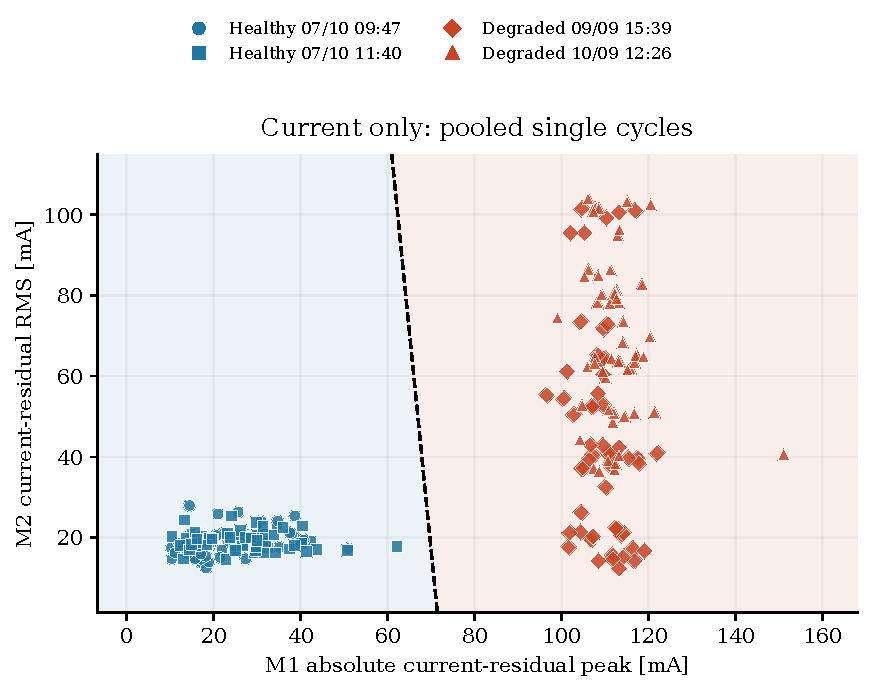
\includegraphics[width=0.98\columnwidth]{Figures/03_pooled_current_lda.pdf}
\caption{Descriptive pooled LDA using M1 absolute current-residual peak
and M2 current-residual RMS. The 216 points represent individual cycles
across all command amplitudes, frequencies and waveforms.
Colours indicate classes and markers indicate runs.
The dashed boundary is fitted to all displayed observations and is
not a cross-validation boundary.}
\label{fig:dof2-lda}
\end{figure}

The complete model comparison, amplitude-specific results and
three-cycle results are provided in Appendix~\ref{app:dof2}.
